 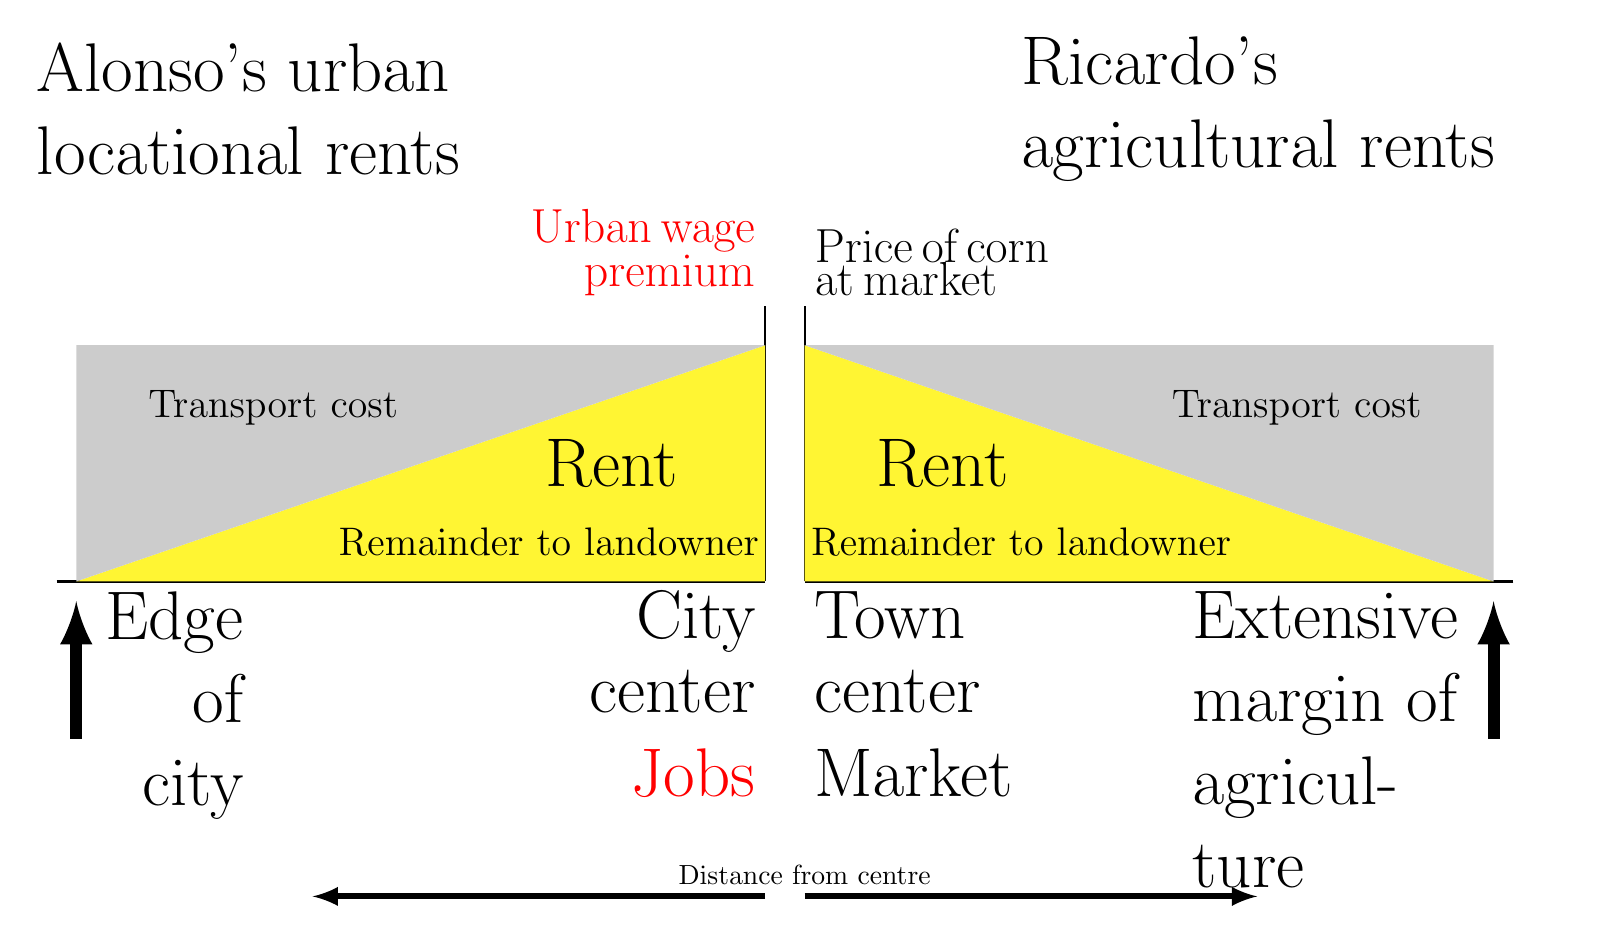
\begin{tikzpicture}[domain=0:2]
 %Combining two RENT figures for one slide
 
%\draw[thick,color=gray,step=.5cm, dashed] (-0.5,-.5) grid (3,3);
%\draw[line width=.01, green ] (0,0) -- (10,0) node[right  ] {Distance};laboutr market
\node at (6.5, 6.) [text width=7cm, font=\Huge ]{Ricardo's\\ agricultural rents};

\node at (.25,0) [below right, text width=4cm, black ]{\Huge Town };
\node at (.25,-1.) [below right, text width=4cm, black ]{\Huge center };
\node at (.25,-2) [below right, text width=4cm, black ]{\Huge Market};
\draw[thick ] (9.25,0)  -- (.25,0);

\draw[thick ] (.25,0)  -- (.25, 3.5)node[above right, text width=3cm, ]{\LARGE Price of corn at market};
\fill[yellow!80]  (.25,0) --(.25,3)--(9,0)node[below left, black, text width=3.7cm, font=\Huge]{ Extensive margin of agriculture} --cycle;
\fill[gray!40] (9,3) --(.25,3)--(9,0) --cycle;

\node  at (2.,1.5)[font=\Huge ]{Rent};
\node  at (3,.5)[font=\Large]{ Remainder to landowner};
\node  at (6.5,2.2){\Large Transport cost};
\draw[latex-, line width=1.5mm] (9,-.25) --(9, -2);
\draw[-latex, line width=.75mm] (.25,-4)node[above]{Distance from centre} --(6,-4);

%\pause

%  ALONSO CITY. negative x]

\node at (-6,6.)[text width=7cm, align=left, font=\Huge ]{ Alonso's  urban \\ locational rents};

\node at (-.25,0) [below left, text width=4cm, black, align=right ]{\Huge City };
\node at (-.25,-1) [below left, text width=4cm, black , align=right]{\Huge center };
\node at (-.25,-2) [below left, text width=4cm, red , align=right]{\Huge Jobs};

\draw[thick ] (-9.25,0)  -- (-.25,0);
\draw[thick ] (-.25,0)  -- (-.25, 3.5)node[above left, text width=3cm, align=right, red]{\LARGE Urban wage premium};
\fill[yellow!80]  (-.25,0) --(-.25,3)--(-9,0)node[below right, text width=2cm, black, align=right, font=\Huge ]{ Edge of city} --cycle;
\fill[gray!40] (-9,3) --(-.25,3)--(-9,0) --cycle;

\node  at (-2.2,1.5)[font=\Huge ]{Rent};
\node  at (-3,.5)[font=\Large]{ Remainder to landowner};

\node  at (-6.5,2.2){\Large Transport cost};
\draw[latex-, line width=1.5mm] (-9,-.25) --(-9, -2);

\draw[-latex, line width=.75mm] (-.25,-4)--(-6,-4);

\end{tikzpicture} 